% Figure 3: two-corner configurations.  Column width.  The two corners used
% are the filled vertices.
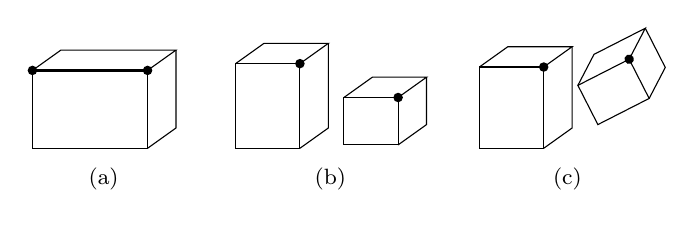
\begin{tikzpicture}[scale=0.86,font=\footnotesize]
  \def\boxdraw#1#2{%
    \draw (0,0) rectangle (#1,#2);
    \draw (0,#2) -- ++(0.42,0.30) -- ++(#1,0) -- (#1,#2);
    \draw (#1,0) -- ++(0.42,0.30) -- ++(0,#2);}
  % (a) connected by an edge
  \begin{scope}[shift={(0,0)}]
    \boxdraw{1.7}{1.15}
    \draw[very thick] (0,1.15) -- (1.7,1.15);
    \fill (0,1.15) circle (2pt) (1.7,1.15) circle (2pt);
    \node at (1.05,-0.45) {(a)};
  \end{scope}
  % (b) one Manhattan frame
  \begin{scope}[shift={(3.0,0)}]
    \boxdraw{0.95}{1.25}
    \fill (0.95,1.25) circle (2pt);
    \begin{scope}[shift={(1.6,0.05)}]
      \boxdraw{0.8}{0.7}
      \fill (0.8,0.7) circle (2pt);
    \end{scope}
    \node at (1.4,-0.45) {(b)};
  \end{scope}
  % (c) independent frames
  \begin{scope}[shift={(6.6,0)}]
    \boxdraw{0.95}{1.2}
    \fill (0.95,1.2) circle (2pt);
    \begin{scope}[shift={(1.75,0.35)},rotate=27]
      \boxdraw{0.85}{0.65}
      \fill (0.85,0.65) circle (2pt);
    \end{scope}
    \node at (1.3,-0.45) {(c)};
  \end{scope}
\end{tikzpicture}
